%%% Exemplo de utilização da classe ITA
%%%
%%%   por        Fábio Fagundes Silveira   -  ffs [at] ita [dot] br
%%%              Benedito C. O. Maciel     -  bcmaciel [at] ita [dot] br
%%%              Giovani Volnei Meinertz   -  giovani [at] ita [dot] br
%%%    	         Hudson Alberto Bode       -  bode [at] ita [dot]br
%%%    	         P. I. Braga de Queiroz    -  pi [at] ita [dot] br
%%%    	         Jorge A. B. Gripp         -  gripp [at] ita [dot] br
%%%    	         Juliano Monte-Mor         -  jamontemor [at] yahoo [dot] com [dot] br
%%%    	         Tarcisio A. B. Gripp      -  tarcisio.gripp [at] gmail [dot] com
%%%    	         
%%%
%%%  IMPORTANTE: O texto contido neste exemplo nao significa absolutamente nada.  :-)
%%%              O intuito aqui eh demonstrar os comandos criados na classe e suas
%%%              respectivas utilizacoes.
%%%
%%%  Tese.tex  2016-08-25
%%%  $HeadURL: http://www.apgita.org.br/apgita/teses-e-latex.php $
%%%
%%% ITALUS
%%% Instituto Tecnológico de Aeronáutica --- ITA, Sao Jose dos Campos, Brasil
%%%                   http://groups.yahoo.com/group/italus/
%%% Discussion list: italus {at} yahoogroups.com
%%%
%++++++++++++++++++++++++++++++++++++++++++++++++++++++++++++++++++++++++++++++
% Para alterar o TIPO DE DOCUMENTO, preencher a linha abaixo \documentclass[?]{?}
%   \documentclass[tg]{ita}			= Trabalho de Graduacao
%   \documentclass[tgfem]{ita}		= Para Engenheiras
%   								msc     		= Dissertacao de Mestrado
%   								mscfem   		= Para Mestras
%   								dsc      		= Tese de Doutorado
%   								dscfem   		= Para Doutoras
%   								quali    		= Exame de Qualificacao
%   								qualifem 		= Exame de Qualificacao para Doutoras
% Para 'Draft Version'/'Versao Preliminar' com data no rodape, adicionar 'dv':
%   \documentclass[dsc, dv]{ita} 
% Para trabalhos em Inglês, adicionar 'eng':
%   \documentclass[dsc, eng]{ita}
%		\documentclass[dsc, eng, dv]{ita}
%++++++++++++++++++++++++++++++++++++++++++++++++++++++++++++++++++++++++++++++
\documentclass[tg, eng, dv]{ita}    % ITA.cls based on standard book.cls 
% Quando alterar a classe, por exemplo de [msc] para [msc, eng]) rode mais uma vez o botão BUILD OUTPUT caso haja erro
\usepackage{booktabs}
\usepackage{ae}
\usepackage{graphicx}
\usepackage{epsfig}
\usepackage{amsmath}
\usepackage{amssymb} 
\usepackage{subfig}
\usepackage{multirow}
\usepackage{float}
\usepackage{lipsum}



%++++++++++++++++++++++++++++++++++++++++++++++++++++++++++++++++++++++++++++++
% Espaçaamento padrão de todo o documento
%++++++++++++++++++++++++++++++++++++++++++++++++++++++++++++++++++++++++++++++
\onehalfspacing

%singlespacing Para um espaçamento simples
%onehalfspacing Para um espaçamento de 1,5
%doublespacing Para um espaaçamento duplo

%++++++++++++++++++++++++++++++++++++++++++++++++++++++++++++++++++++++++++++++
% Identificacoes (se o trabalho for em inglês, insira os dados em inglês)
% Para entradas abreviadas de Professora (Profa.) em português escreva: Prof$^\textnormal{a}$.
%++++++++++++++++++++++++++++++++++++++++++++++++++++++++++++++++++++++++++++++
\course{Computer Engineering} % Programa de PG ou Curso de Graduação
% \area{Sistemas Aeroespaciais e Mecatrônica} % área de concentração na PG (Não utilizado no caso de TG)

% Autor do trabalho: Nome Sobrenome
\authorgender{masc} %sexo: masc ou fem
\author{Heládio Sampaio}{Lopes}
\itaauthoraddress{H8A St., 113}{12228-460}{São José dos Campos--SP}

% Titulo da Tese/Dissertação
\title{Natural Language Processing for Trend Forecasting}

% Orientador
\advisorgender{masc} % masc ou fem
\advisor{Prof. Dr.}{Filipe Alves Neto Verri}{ITA}

% Coorientador (Caso no haja coorientador, colocar ambas as variveis \coadvisorgender e \coadvisor comentadas, com um % na frente)
% \coadvisorgender{fem}									% masc ou fem
% \coadvisor{~Dr$^\textnormal{a}$.}{Rosa de Fátima Cruz Marques}{IAE}

% Pró-reitor da Pós-graduação
% \bossgender{masc}												% masc ou fem
% \boss{Prof.~Dr.}{John von Neumann}

%Coordenador do curso no caso de TG
\bosscoursegender{masc}									% masc ou fem
\bosscourse{}{Inaldo Capistrano Costa}

% Palavras-Chaves informadas pela Biblioteca -> utilizada na CIP
\kwcip{Natural Language Processing}
\kwcip{Deep Learning}
\kwcip{Machine Learning}

% membros da banca examinadora

% \examiner{Prof. Dr.}{Alan Turing}{Presidente}{ITA}
% \examiner{Prof. Dr.}{Linus Torwald}{}{UXXX}
% \examiner{Prof. Dr.}{Richard Stallman}{}{UYYY}
% \examiner{Prof. Dr.}{Donald Duck}{}{DYSNEY}
% \examiner{Prof. Dr.}{Mickey Mouse}{}{DISNEY}

% Data da defesa (més em maiúsculo, se trabalho em inglês, e minusculo se trabalho em português) 
\date{19}{JUNE}{2020}

% Número CDU - (somente para TG)
\cdu{621.38}

% Glossario
\makeglossary
\frontmatter

\begin{document}	
% Folha de Rosto e Capa para o caso do TG
\maketitle

% Dedicatoria: Nao esqueca essa secao  ... :-)
\begin{itadedication}

\end{itadedication}

% Agradecimentos
\begin{itathanks}
Thank you
\end{itathanks}

% Epígrafe
\thispagestyle{empty}
\ifhyperref\pdfbookmark[0]{\nameepigraphe}{epigrafe}\fi
\begin{flushright}
\begin{spacing}{1}
\mbox{}\vfill
{\sffamily\itshape
``That's All Folks''\\}
--- Looney Tunes, \textsc{}
\end{spacing}
\end{flushright}

% Resumo
\begin{abstract}
\noindent
Com avanço cientifico-tecnológico em escalas globais, a disponibilidade de dados para serem analisados cresce de maneira exponencial. A partir desse crescimento acelerado, técnicas de inteligência artificial, como o Processamento de Linguagem Natural (PLN), ajudam a automatizar o processo de se extrair informação de documentos.  Com intuito de realizar previsões sobre as tendências que surgirão em meio ao crescimento de dados, é possível utilizar técnicas de modelagem de tópicos para agrupar documentos em temas semelhantes e estudar a incidência temporal desses temas.

Assim, este trabalho busca aplicar técnicas de PLN combinadas com aprendizado supervisionado para agrupar documentos em um conjunto de temas e a partir disso aprender a identificá-los em novos documentos em um período futuro. Utilizando publicações cientificas da conferência de Sistemas de Processamento de Informação Neural, fomos capazes de modelar essa tarefa e obter bons resultados. Também estudamos a capacidade dos classificadores de manter desempenho satisfatório com o passar do tempo.

\end{abstract}

% Abstract
\begin{englishabstract}
\noindent
With scientific and technological advances on global scales, the availability of data to be analyzed grows exponentially. Based on this accelerated growth, artificial intelligence techniques, such as Natural Language Processing (NLP), increasingly help to automate the process of extracting information from documents. In order to make predictions about the trends that will arise from data growth, it is possible to use topic modeling techniques to group documents on similar clusters and study the temporal incidence of those topics.

Thereby, this work aims to apply NLP techniques combined with supervised learning to group documents into a set of themes and from there learn to identify them in new documents in a future period. Using scientific publications from the Conference on Neural Information Processing Systems, we were able to model this task and obtain good results, \dots
% TODO: terminar o texto para ficar coerente com a modificação no texto em português

\end{englishabstract}

% Lista de figuras
\listoffigures %opcional

% Lista de tabelas
\listoftables %opcional

% Lista de abreviaturas
\listofabbreviations
\begin{longtable}{ll}
	AI     & Artificial Intelligence                   \\
	BoW    & Bag of Words                              \\
	CBOW   & Continuous Bag of Words                   \\
	FN     & False Negative                            \\
	FP     & False Positive                            \\
	IT     & Information Technology                    \\
	LDA    & Latent Dirichelt Allocation               \\
	LOWESS & Locally Weighted Scatterplot Smoothing    \\
	ML     & Machine Learning                          \\
	NIPS   & Neural Information Processing Systems     \\
	NLP    & Natural Language Processing               \\
	NPMI   & Normalized Pointwise Mutual Information   \\
	OLS    & Ordinary Least Squares                    \\
	TF-IDF & Term Frequency Inverse Document Frequency \\
	TN     & True Negative                             \\
	TP     & True Positive                             \\
\end{longtable}

 %opcional

% Lista de simbolos
\listofsymbols
%\begin{longtable}{ll}
%$a$ & Distncia\\
%$\textbf{a}$ & Vetor de distncias\\
%$\textbf{e}_{j}$ & Vetor unitrio de dimenso $n$ e com o $j$-simo componente igual a $1$ \\
%$\textbf{K}$ & Matriz de rigidez\\
%$m_1$ & Massa do cumpim\\
%$\delta_{k-k_f}$ & Delta de Kronecker no instante $k_f$\\
%
%\end{longtable}
%
 %opcional

% Sumario
\tableofcontents

\mainmatter
% Os capitulos comecam aqui

\chapter{Introduction}\label{chap:intro}
Recently, the growth of artificial intelligence has been helping us to solve problems in most various areas, including linguistics. With natural language processing techniques, computers can process text in order to extract information faster than humans.

\section{Motivation}

%Every kind of expression, verbal or in writing, brings us much information to be interpreted. Whether the topic is chosen, the tone used, the choice of words, everything can be interpreted, and then generate some valuable information. Over the years, more and more knowledge is generated and we humans are unable to process such an amount of information. Natural Language Processing emerges as a technology capable of assisting us in this hard task.

%\citeonline{state_of_the_art} defines Natural Language Processing, abbreviated by NLP, as a branch of artificial intelligence capable of making computers comprehend and extract information from human language. NLP can perform a lot of tasks, such as identifying different topics for a set of documents, classifying texts on predefined subjects, and beyond that extract the sentiment to know what people are saying about something.

%The topic discovery was widely explored in the literature, \citeonline{hurtado2016topic} and \citeonline{jelodar2020deep} use it to group, respectively, papers abstracts and comments in social media in similar clusters. In a long period, it is possible to analyze how these founded topics behave through time and make predictions about the near future.

Every kind of expression, verbal or in writing, brings us much information to be interpreted. Whether the topic is chosen, the tone used, the choice of words, everything can be interpreted, and then generate some valuable information.

Over the years, more and more knowledge is generated and we humans are unable to process such an amount of information. A study made by \citeonline{beath2012finding} reveals that the enterprises' volume of data is expanding by 35\%-50\% every year, including textual data. Despite this, they also find that the companies could not extract information from this huge amount of data.

In that way, extracting valuable information from this data has become more and more an important skill. Therefore, Natural Language Processing emerges as a technology capable of assisting us in the task of deal with textual data.

\citeonline{khurana2017natural} defines Natural Language Processing, abbreviated by NLP, as a branch of artificial intelligence capable of making computers comprehend and extract information from human language.
In fact, NLP can perform simple tasks but not quite scalable for a human, such as translate text from one language to another, identify different topics for a set of documents, classify text on predefined subjects, and beyond that extract the sentiment to know what people are saying about something.

% Falar sobre alexa, google assistente e siri.
In recent years a particular kind of NLP application is drawing a lot of attention. The voice assistants like Siri, Cortana, Alexa and Google Assistant are the hot AI topics of the moment. Together, all digital assistants attempted to answer more and more questions each year, \cite{kailakrayewski2019}.

\newpage
In our particular scope, the topic discovery was widely explored in the literature. \citeonline{hurtado2016topic} and \citeonline{jelodar2020deep} use it to group, respectively, papers abstracts and comments in social media in similar clusters. The first one uses it to study the topics' evolution and correlation between the founded topics. In contrast, the second group comments to analyze the general sentiment about them.

However, these related works apply topic modeling only for static analysis. In this work context, we are seeking a real-time application that will keep receiving news in a continuous process. Thus, redo the topic discovery process will demand an expensive computational cost, besides the human effort to label the topics. To avoid the rework of modeling the documents in topics, a classification-based system will be proposed, for a future development of a real-time application is possible.


\section{Objective}

%Curious about the fast world's evolution, this work aims to implement Natural Language Processing techniques to propose a framework capable of modeling in real-time the topics' evolution over the years. With this in mind, evaluate the ability of those models to make predictions about future trends.

Curious about the fast world's evolution, this work aims to implement Natural Language Processing techniques to propose a framework capable of modeling in real-time the topics' evolution over time, using an annual granularity. 
With this in mind, we must evaluate the ability of those models in modeling the themes occurrence over the years.

By the end of this work, a series of tasks must be done. First, we must normalize the documents to segment them into time-ordered subsets, \textit{Past}, \textit{Present} and \textit{Future}, respectively. With the eldest subset, we must find meaningful subjects to train classification models based on these topics. Then, evaluate the predictions for \textit{Present} set and how the models' performance degenerates over the years.

% Esta seção deve conter:
%   - Objetivo geral: propor um framework para aprender evolução de tópicos em texto em
%     linguagem natural ao longo do tempo.
%   - Objetivos específicos:
%     a) Propor a divisão da base de dados em diferentes conjuntos
%     b) Encontrar os tópicos no passado
%     c) Treinar classificadores
%     d) Avaliar o desempenho no presente
%     e) Avaliar a degeneração do desempenho

%\section{Objective}
%
%As already discussed, we want to build models capable of making predictions regarding the evolution of discovered topics in a set of documents. We also want to find topics in real-time at each received document without having to redo the topic discovery process. Then, by the end of this work, we must have performed the tasks listed below.
%
%\begin{itemize}
%	\item Find a database long enough, over several years;
%	\item Perform all necessary treatment steps to normalize the documents' texts;
%	\item Find meaningful topics in a subset from the original database;
%	\item Create a topic classifier to find out if a document addresses any topic of interest;
%	\item Model topic evolution to evaluate the forecast accuracy.
%\end{itemize}

\section{Organization of this work}

The remaining of this work is organized as follows: Chapter \ref{chap:literature} will cover the theory behind Natural Language Processing and basics Classification. Chapter \ref{chap:related} will describe some previous works which use topic discovery and trend forecast. Chapter \ref{chap:materials} will better explain the problem and the methodology that will be used to handle it. Chapter \ref{chap:results} will show the discovered results for the proposed experiment and some discussion about them. Finally, Chapter \ref{chap:conclusion} will present some conclusions and suggestions for future work.


\chapter{Background and Literature Review}\label{chap:background}
% Introduzir, com base em referências, o problema que será abordado no decorrer do TG. 


\section{Definition}


\section{Applications}



\chapter{Natural Language Processing}\label{chap:nlp}
\section{Text Processing Techniques}

The key task to several machine learning problems consist in make a good data processing before applying any model. A clean data set can allow a model to increase its performance in the learning process, making a better identification in the patterns present in the variables. Hence, in the next sections, it will be discussed a few techniques to clear the text and prepare it for ML algorithms.

\subsection{Normalization}
%https://www.kdnuggets.com/2017/12/general-approach-preprocessing-text-data.html

There is no right way to normalize text, this process has it is really important to put all text in the same level. A normalization process has a series of steps to be followed sequentially, all of then can be seen as 4 big tasks: stemming, lemmatization, stop words removal and everything else.

\begin{enumerate}
	\item Stemming: Is the process of reduce inflected words to a primitive form, the stem. This method is able to remove the word's affixes to capture its base meaning, and still reducing the number of variations to save memory space. Figure \ref{fig:stemming} shows how some inflections for "connect" can be converted to its root form.
		
	\begin{figure}[h!]
		\centering
		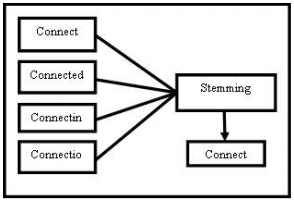
\includegraphics[width=0.45\linewidth]{01.Chapters/03.NLP/stemming}
		\caption{Stemming process for connect variations \cite{vijayarani2015preprocessing}.}
		\label{fig:stemming}
	\end{figure}
	
	% stemming algorithms
	
	\item Lemmatization: similar to stemming, this step also reduce words to some primitive form, but with a little improvement. Lemmatization can returns the words to his dictionary form, based on its part of speech context. So it is possible to discriminate words with the same spelling but different meanings depending on the context. 	
	
	\item Remove stop words:
	Many words can occurs a several times in a document without add any meaningful information, such as \textit{the}, \textit{is}, \textit{at}, \textit{which}, and \textit{on}. Their high frequency can be seen as an obstacle to perform good results on NLP models, \cite{kannan2014preprocessing}. 

	There are some types to remove stop words, most of then based on evaluating the frequency of words in text, for more information see \cite{x}. But the classic and easier method is based on using a pre-compiled list of know words and removing then from text.
	
	\item Everything else:
	Differently from the previous steps, the last one doesn't need any grammar rules or even a frequency analysis, it's purely text manipulation. It involves set all character to lowercase; remove numbers or convert then to word form; remove punctuation; expand contractions; convert special characters to ASCII form; and any other conversion needed.		 	
\end{enumerate}

\subsection{Tokenization}
	Once the data is normalized, we need to know how to represent it. The tokenization process consists in splitting longer strings into meaningful small pieces called tokens. The most common way to tokenize a text is chunking it the into words, ie, given a piece of text the tokenize process will return a list of words. 
	
	
\subsection{Bag of Words}
	The machine learning algorithms take numerical features as input, hence, it will bee necessary to represent the text in numerical form. With the Bag of Words model we can represent in matrix form a set of documents.
	 	
	With the tokenization output we will have the lists representations for all documents in the data set. These lists can be interpreted as vectors over the vector space of all unique tokens, also called by vocabulary. So, for a given sentence, we mark how many times its words appears in the list indexes where each entry corresponds to a word in the vocabulary. The Figure \ref{fig:bag-of-words} show a simple example of how three sentences can be represented with BoW model.
	
	
	\begin{figure}[h!]
		\centering
		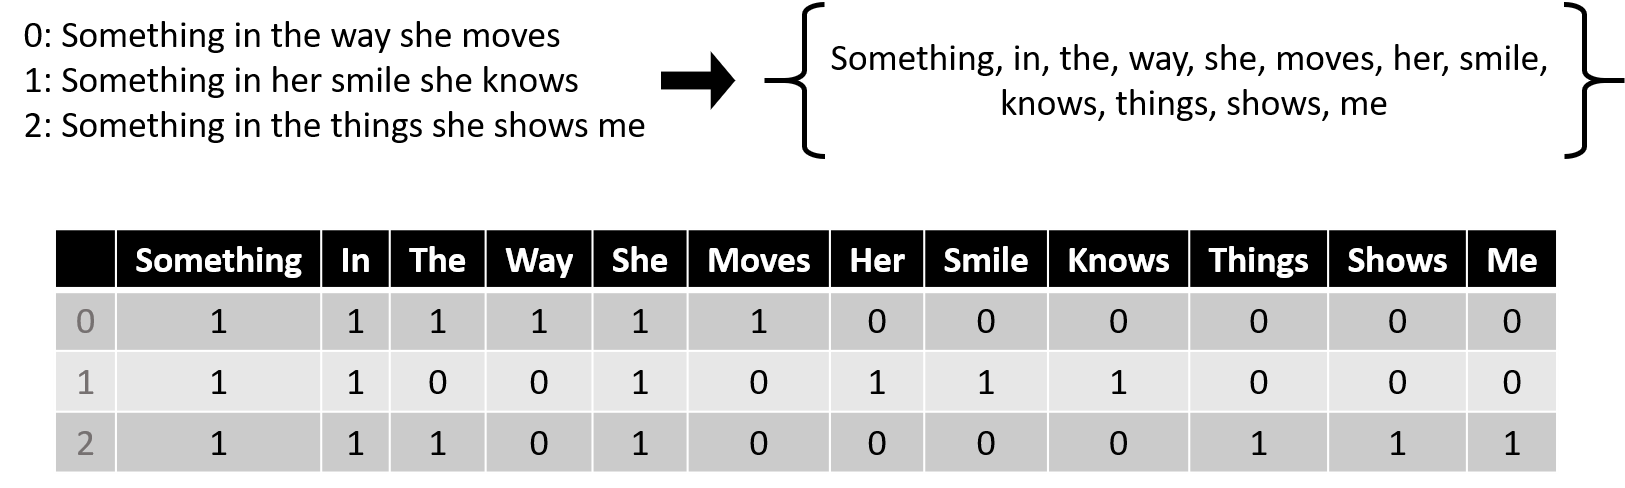
\includegraphics[width=\linewidth]{01.Chapters/03.NLP/bag-of-words}
		\caption{Bag of Words example.}
		\label{fig:bag-of-words}
	\end{figure}
	

\subsection{TF-IDF}

	Term Frequency Inverse Document Frequency, TF-IDF for short, it is applied to a BoW to determine the relative frequency for words in a specific document when compared to the inverse proportion of that word over all documents in the collection. So, it can be determined how important are the words in a specific document. 
		
	From BoW, for the $i^{th}$ vocabulary's word in the $j^{th}$ document, its TF-IDF weight, $w_{i,j}$, can be calculated with Equation \ref{eq:tf-idf}.
	
	\begin{equation}
		\label{eq:tf-idf}
		w_{i, j} = tf_{i, j} \times \log\left(\dfrac{N}{df_{i}}\right)
	\end{equation}
	
	Where, the term frequency, $tf_{i, j}$, is how many time $i^{th}$ word appears in the $j^{th}$ document. The document frequency, $df_{i}$, is the number of documents in which th $i_{th}$ vocabulary words is present. And, finally, $N$ is the size of the document collection, with a large number of documents this term can explodes, so the logarithmic function is applied to dampen this effect.
	
		
\section{Word Embedding}

	The vectorization methods such as BoW and TF-IDF can be very useful, but they can not represent the words context. This means that the same words used in different contexts have the same representation, just as different words used with the same meaning are represented differently. Besides that, an one-hot encoding method, like BoW, presents a very sparse representation with high dimensionality. 
	
	The Word Embedding is a technique to represent words in vectors capable of capture the words context in a document. It is also able to smooth the high 
	dimensionality effect by using much more compact vector to represent the words.	


\section{Topic Modeling}

	

\section{Topic Classification}



\chapter{Deep Learning}\label{chap:deep}
\section{Neuron}


\section{Perceptron and Activation Functions}


\section{Loss Functions}


\section{Optimization}

	

%\chapter{Methodology}\label{chap:methodoogy}
%\input{01.Chapters/05.Methodology/methodology}
%
%\chapter{Results and Discussions}\label{chap:results}
%In the last chapter, we detailed all the methodology steps behind the experimentation. In this one, we will show the proper results obtained by the topic modeling and classification steps.

\section{Topic Modeling}

In this first section, the results are related to the topic modeling step, divided into four stages: the vocabulary selection; the topic coherence optimization; applying LDA in past and present set; and the combination of topics from the past and future.

\subsection{Vocabulary Selection}

After the normalization, we had performed the Luhn's cut in order to remove words with document frequency higher than 60\% and words that appear in less than 5 documents. The cut was performed in both \textit{Past} and \textit{Present} sets, the Table \ref{tab:vocabulary} shows a brief description for the vocabularies dimension before and after the selection, and for their intersection.

\begin{table}[h!]
	\centering
	\caption{Vocabulary description.}
	\label{tab:vocabulary}
	\begin{tabular}{l|cccc}
		\toprule
		          &  \textbf{Raw}  & \textbf{High DF} & \textbf{Low DF} & \textbf{Filtered} \\ \midrule
		Past      & 77512 &   104   & 65480  &  11928   \\
		Present   & 90122 &   183   & 70356  &  19583   \\
		Intersect &   -   &    -    &   -    &   9745   \\ \bottomrule
	\end{tabular}
\end{table}

With this cut, words like ``abstract'', ``show'' and ``reference'' were removed from the vocabulary. They are quite common in this type of scientific publication and are not relevant for analysis. The low frequency includes very specific words and mostly misspellings.

\subsection{Topic Coherence Optimization}

To find the best topic model for our data, an hyperparameter optimization has been performed over the three LDA parameters: $\alpha \in \left\{0.1, 0.5, 1\right\}$, $\beta \in \left\{0.05, 0.1, 0.5, 1\right\}$ and $K \in \left\{10, 15, 20, 25, 30, 35, 40\right\}$. The dataset used was the \textit{Past} set with its vocabulary as described in the previous section. Figure \ref{fig:coherence-optimization} shows the coherence score $C_{\text{V}}$ by the number of topics for the main $\alpha$ and $\beta$ combinations.

\begin{figure}[h!]
	\begin{subfigure}{0.49\textwidth}
		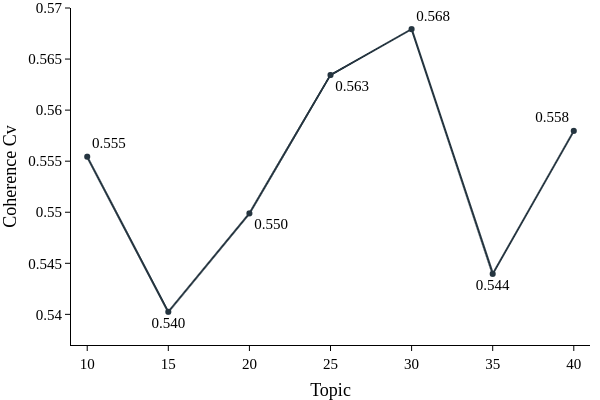
\includegraphics[width=\linewidth]{01.Chapters/05.Results/01_Topic_Cv_A:0.5| B:1.00}
		\caption{$\alpha = 0.5$ and $\beta = 1.0$.}
	\end{subfigure}%
	\hfill
	\begin{subfigure}{0.49\textwidth}
		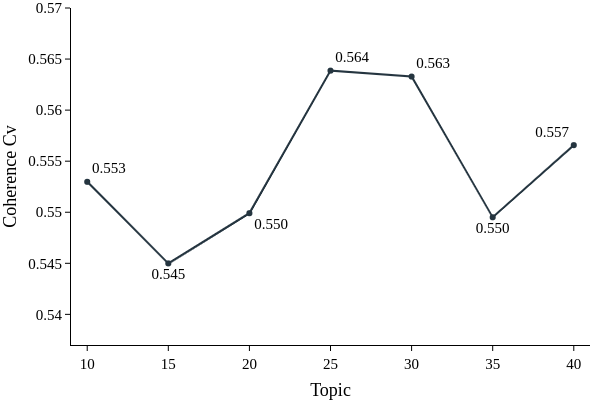
\includegraphics[width=\linewidth]{01.Chapters/05.Results/02_Topic_Cv_A:0.1| B:1.00}
		\caption{$\alpha = 0.1$ and $\beta = 1.0$.}
	\end{subfigure}%
	\vfill
	\begin{subfigure}{0.49\textwidth}
		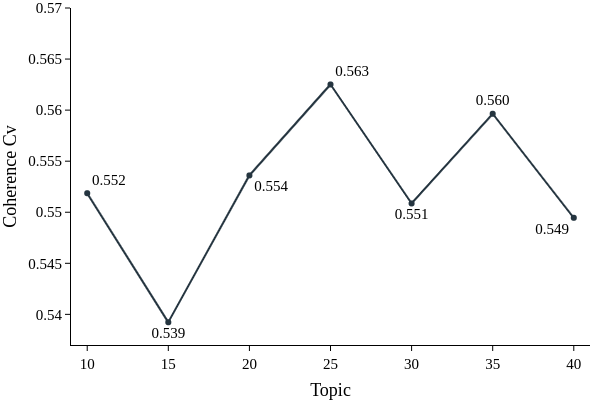
\includegraphics[width=\linewidth]{01.Chapters/05.Results/03_Topic_Cv_A:1.0| B:1.00}
		\caption{$\alpha = 1.0$ and $\beta = 1.0$.}
	\end{subfigure}%
	\hfill
	\begin{subfigure}{0.49\textwidth}
		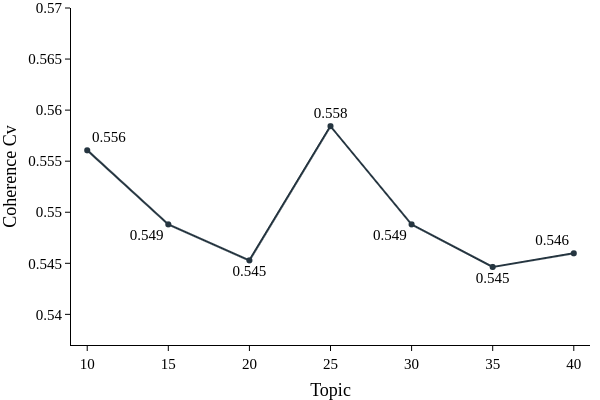
\includegraphics[width=\linewidth]{01.Chapters/05.Results/04_Topic_Cv_A:1.0| B:0.10}
		\caption{$\alpha = 1.0$ and $\beta = 0.1$.}
	\end{subfigure}%
	\caption{Topic Coherence Optimization.}
	\label{fig:coherence-optimization}
\end{figure}

Although the combination for $\alpha = 0.5$ and $\beta = 1.0$ has it maximum for $30$ topics, we can clearly detect a maximum trend for $25$ topics. From the application point of view, the smaller the number of topics the better for a human to follow their evolution. In this manner, we decided on $25$ topics to proceed with the experiment, with this value for $K$, the $\alpha$ and $\beta$ parameters with the best coherence score are $0.1$ and $1.0$, respectively.

\subsection{Finding Topics}

At this stage we had performed the LDA algorithm over the \textit{Past} and \textit{Present} sets, with the parameters established in the previous stage and their respective vocabularies, to find their topics. After the modeling the \textit{Present} model has presented a coherence of $0.614$, this indicates that the \textit{Present} model is slightly better than the \textit{Past} one.

\subsubsection{Past}

Figure \ref{fig:past-wordcloud} shows some word clouds for \textit{Past} topics that are easier to identify what they talk about. For example, topic 0 talks about image recognition, topic 10 clearly is about reinforcement learning, topic 16 can be about supervised learning, and topic 19 about facial recognition. To assess all the topics in more detail check Appendix \ref{apdx:past}.

\begin{figure}[h!]
	\begin{subfigure}{0.49\textwidth}
		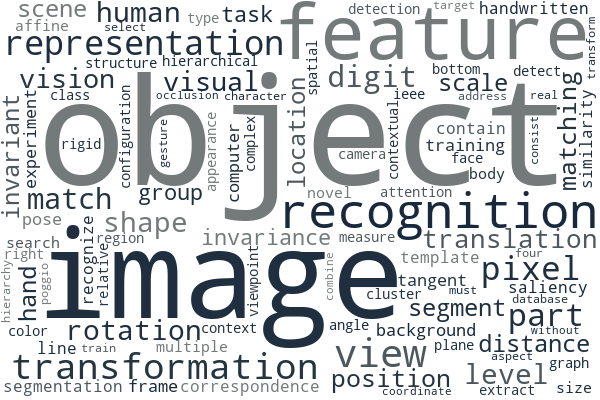
\includegraphics[width=\linewidth]{01.Chapters/05.Results/past_00}
		\caption{Past topic number 0.}
	\end{subfigure}%
	\hfill
	\begin{subfigure}{0.49\textwidth}
		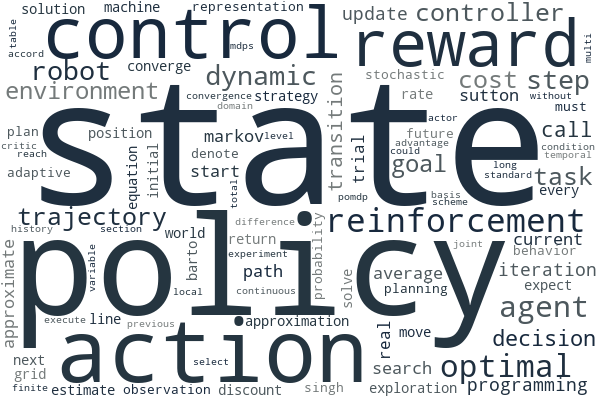
\includegraphics[width=\linewidth]{01.Chapters/05.Results/past_10}
		\caption{Past topic number 10.}
	\end{subfigure}%
	\vfill
	\begin{subfigure}{0.49\textwidth}
		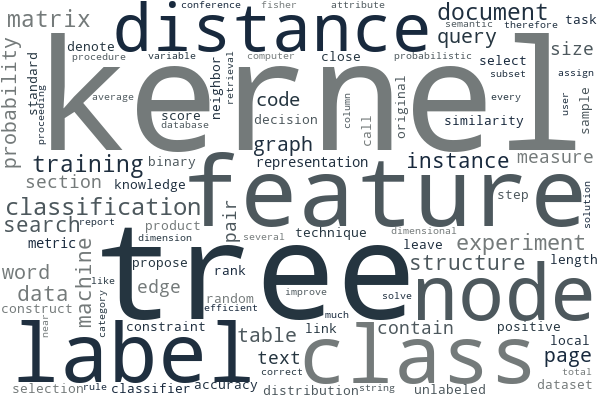
\includegraphics[width=\linewidth]{01.Chapters/05.Results/past_16}
		\caption{Past topic number 16.}
	\end{subfigure}%
	\hfill
	\begin{subfigure}{0.49\textwidth}
		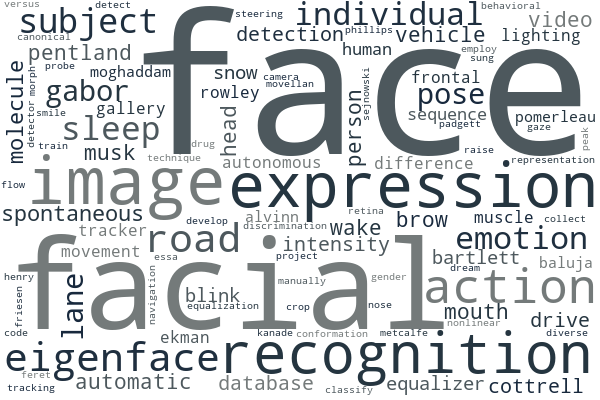
\includegraphics[width=\linewidth]{01.Chapters/05.Results/past_19}
		\caption{Past topic number 19.}
	\end{subfigure}%
	\caption{\textit{Past} topics wordclouds.}
	\label{fig:past-wordcloud}
\end{figure}

Besides getting the topics we also have the distribution of the documents of topics. Using these distributions we had labeled the documents as positive or negative for the topics with a threshold of $1 / K$, i.e., for a document covers a given topic his probability has to be at least $0.08$. This probability guarantees, by the pigeonhole principle, that the documents have at least one topic.

Figure \ref{fig:past-topic-dist} shows the distribution of topics over the documents. In Figure \ref{fig:past-percentage-bar} we have the percentage of documents that is about the 25 past topics, Figure \ref{fig:past-percentage-hist} shows the histogram for these percentages, each bin with $2.5\%$. According to the figures, none of the topics are in more than $50\%$ of the documents, some of them are present in less than $2.5\%$, but mostly they are distributed between $10\%$ and $35\%$.

\begin{figure}[h!]
	\begin{subfigure}{0.49\textwidth}
		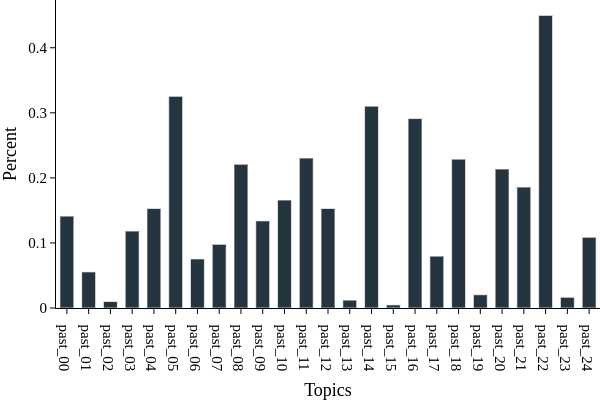
\includegraphics[width=\linewidth]{01.Chapters/05.Results/past-percentage-bar}
		\caption{Percentage of documents with topics.}
		\label{fig:past-percentage-bar}
	\end{subfigure}%
	\hfill
	\begin{subfigure}{0.49\textwidth}
		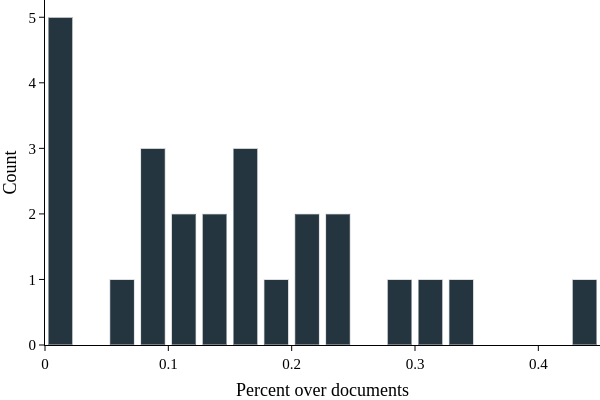
\includegraphics[width=\linewidth]{01.Chapters/05.Results/past-percentage-hist}
		\caption{Histogram for the topic percentages.}
		\label{fig:past-percentage-hist}
	\end{subfigure}%
	\caption{Distribution of topics over the documents.}
	\label{fig:past-topic-dist}
\end{figure}

Figure \ref{fig:past-topic-per-doc} shows the distribution of topics in each document. This histogram shows that most documents have more than one topic, a few have only one topic, even fewer have more than 7, and none document has more than 10 topics.

\begin{figure}[h!]
	\centering
	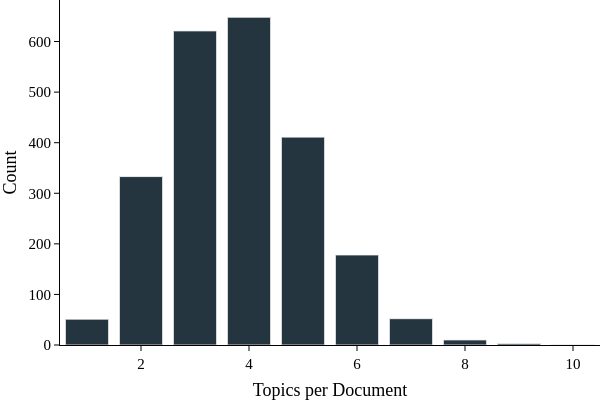
\includegraphics[width=0.6\linewidth]{01.Chapters/05.Results/past-topic-per-doc}
	\caption{Histogram for the number of topics per document.}
	\label{fig:past-topic-per-doc}
\end{figure}


\subsubsection{Present}

Figure \ref{fig:pres-wordcloud} shows some word clouds for \textit{Present} topics that are easier to identify what they talk. For example, topic 0 clearly is about NLP and topic modeling, topic 13 is about clustering, topic 16 can be about statistical inference, and topic 24 about classification. To access all the topics in more detail check Appendix \ref{apdx:present}.

\clearpage
\begin{figure}[h!]
	\begin{subfigure}{0.49\textwidth}
		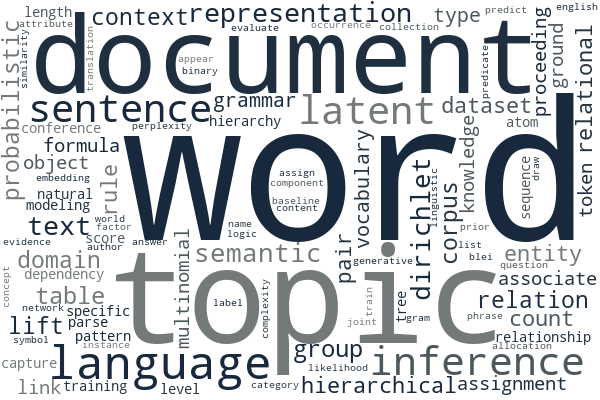
\includegraphics[width=\linewidth]{01.Chapters/05.Results/pres_00}
		\caption{Present topic number 0.}
	\end{subfigure}%
	\hfill
	\begin{subfigure}{0.49\textwidth}
		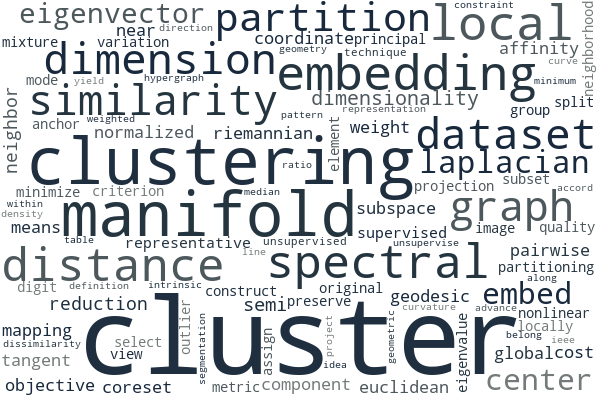
\includegraphics[width=\linewidth]{01.Chapters/05.Results/pres_13}
		\caption{Present topic number 13.}
	\end{subfigure}%
	\vfill
	\begin{subfigure}{0.49\textwidth}
		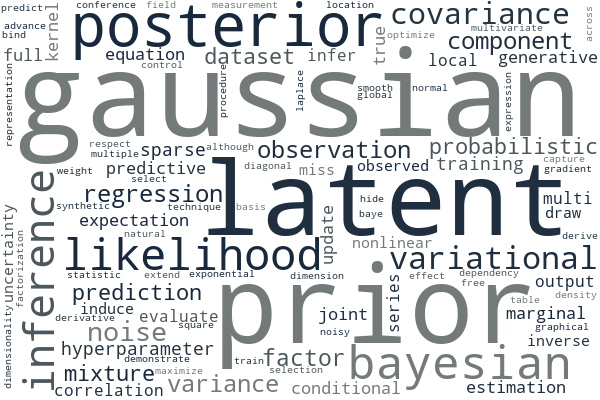
\includegraphics[width=\linewidth]{01.Chapters/05.Results/pres_16}
		\caption{Present topic number 16.}
	\end{subfigure}%
	\hfill
	\begin{subfigure}{0.49\textwidth}
		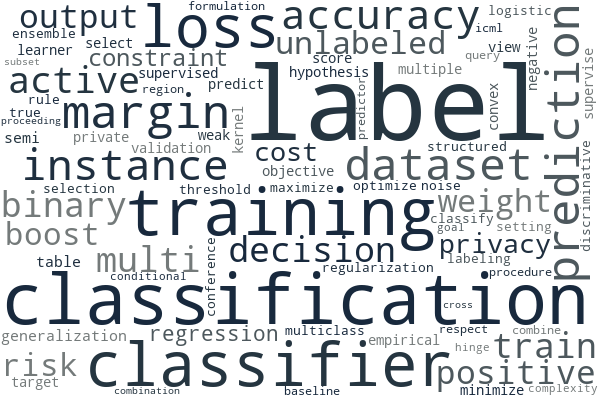
\includegraphics[width=\linewidth]{01.Chapters/05.Results/pres_24}
		\caption{Present topic number 24.}
	\end{subfigure}%
	\caption{\textit{Present} topics wordclouds.}
	\label{fig:pres-wordcloud}
\end{figure}

Figures \ref{fig:pres-topic-dist} and \ref{fig:pres-topic-per-doc} have the same idea as the Figures \ref{fig:past-topic-dist} and \ref{fig:past-topic-per-doc}. The \ref{fig:pres-topic-dist} shows that the topics are well distributed over the documents, the topic present in more documents is about $35\%$ of them. Figure \ref{fig:pres-topic-per-doc} shows the distribution of \textit{present} topics over the docuements, similarly to the \textit{past} distribution, the documents have mostly about 3 and 4 topics and none of then have more than 10 topics.

\begin{figure}[h!]
	\begin{subfigure}{0.49\textwidth}
		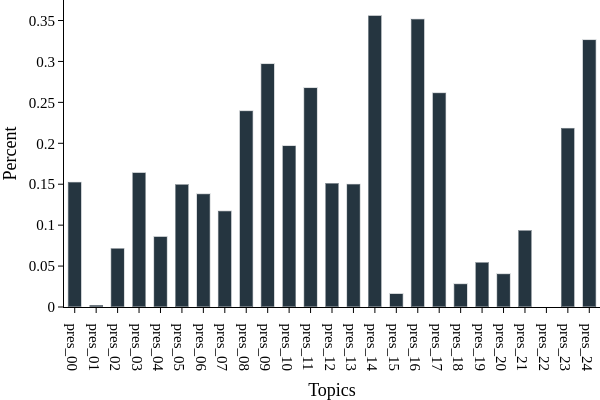
\includegraphics[width=\linewidth]{01.Chapters/05.Results/pres-percentage-bar}
		\caption{Percentage of documents with topics.}
		\label{fig:pres-percentage-bar}
	\end{subfigure}%
	\hfill
	\begin{subfigure}{0.49\textwidth}
		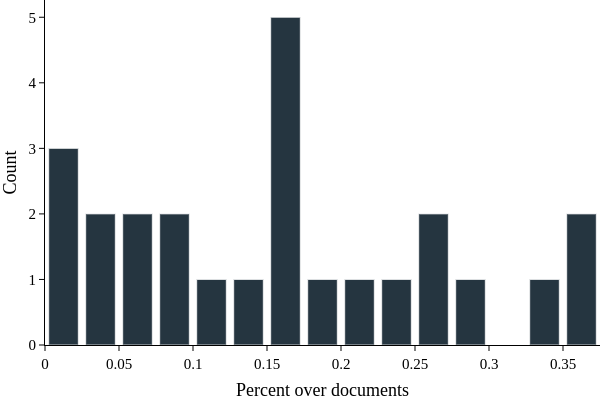
\includegraphics[width=\linewidth]{01.Chapters/05.Results/pres-percentage-hist}
		\caption{Histogram for the topic percentages.}
		\label{fig:pres-percentage-hist}
	\end{subfigure}%
	\caption{Distribution of topics over the documents.}
	\label{fig:pres-topic-dist}
\end{figure}

\begin{figure}[h!]
	\centering
	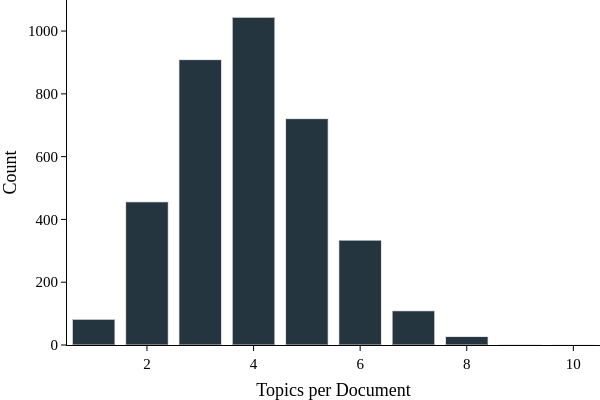
\includegraphics[width=0.55\linewidth]{01.Chapters/05.Results/pres-topic-per-doc}
	\caption{Histogram for the number of topics per document.}
	\label{fig:pres-topic-per-doc}
\end{figure}

\subsection{Past-Present Correspondence}

With the \textit{past} and \textit{present} topics defined, the similarity metrics described in section \ref{sec:material-combination} were applied to obtain the topic correspondence. For $\text{Sim}_{1}$, we use the top 50 words, i.e., $N=50$. As $\text{Sim}_{1}$ and $\text{Sim}_{2}$ are negatively correlated, to aggregate then, we divide $\text{Sim}_{1}$ for $\text{Sim}_{2}$ to capture the best from both metrics. Table \ref{tab:correspondence-score} illustrates the main correspondences between \textit{past} and \textit{present} topics.

\begin{table}[h!]
	\centering
	\caption{Main association for \textit{past} and \textit{present} topics.}
	\label{tab:correspondence-score}
	\begin{tabular}{cc|ccc}
		\toprule
		\textbf{Past} & \textbf{Present} & \textbf{$\text{Sim}_{1}$} & \textbf{$\text{Sim}_{2}$} & \textbf{$\text{Sim}_{1} / \text{Sim}_{2}$} \\ \midrule
		 11 &   06 &   58\% &   0.026 &   22.39 \\
		 10 &   05 &   56\% &   0.031 &   18.23 \\
		 14 &   16 &   44\% &   0.040 &   11.11 \\
		 20 &   09 &   38\% &   0.036 &   10.56 \\
		 18 &   11 &   40\% &   0.043 &    9.35 \\
		 07 &   12 &   34\% &   0.038 &    8.91 \\
		 04 &   02 &   54\% &   0.061 &    8.82 \\
		 00 &   08 &   46\% &   0.055 &    8.36 \\
		 05 &   03 &   32\% &   0.047 &    6.83 \\
		 22 &   07 &   36\% &   0.057 &    6.27 \\ \bottomrule
	\end{tabular}
\end{table}

By aggregating the two metrics, we are choosing topics whose common word distribution is similar while giving priority to topics with the most similar top words. For example, take the correspondence 18-11 and 07-12, the second one is the closest in terms of word distribution, but the first has the top 50 more similar making this correspondence stronger. Table \ref{tab:correspondence-words} shows the intersection for those top 10 topic correspondences.

\begin{table}[h!]
	\centering
	\caption{Words intersection for the main correspondence.}
	\label{tab:correspondence-words}
	\begin{tabular}{cc|lllll}
		\toprule
		\textbf{Present} & \textbf{Past} & \multicolumn{5}{c}{\textbf{Words}} \\ \midrule
		11 & 06 & neuron   & spike      & cell        & response   & stimulus      \\
		10 & 05 & policy   & action     & control     & reward     & reinforcement \\
		14 & 16 & gaussian & mixture    & likelihood  & prior      & bayesian      \\
		20 & 09 & gradient & constraint & convergence & update     & cost          \\
		18 & 11 & bound    & theorem    & loss        & bind       & proof         \\
		07 & 12 & subject  & stimulus   & human       & response   & trial         \\
		04 & 02 & signal   & filter     & noise       & frequency  & channel       \\
		00 & 08 & object   & image      & recognition & pixel      & shape         \\
		05 & 03 & markov   & inference  & sequence    & likelihood & bayesian      \\
		22 & 07 & unit     & training   & layer       & train      & hide          \\ \bottomrule
	\end{tabular}
\end{table}

Through the intersections we see that some \textit{past} topics continued in the \textit{present}. For example, the correspondence 10-05 talks about reinforcement learning, and 22-07 is about deep learning. From that, we evaluate how the models of the \textit{past} behave with the \textit{present}.

\section{Document Classification}

This section will cover the results behind the classification model. First, the training process and model selection with the \textit{Past} set, then, the evaluation of those models at \textit{Present} according to the combination of topics.

\subsection{Model Selection}

%With the documents labeled, we now have our \textit{Labeled Past} dataset. From that, we can train a binary classification model for each topic. For the classification was performed cross-validation with 10 folds for each combination of vectorization + model, the raw results for those models are in Appendix \ref{apdx:classification}.

We now have the \textit{Labeled Past} dataset. From that, we can train a classification model for each topic. For this was performed cross-validation with 10 folds for each combination of vectorization + model, the raw results for those models are in Appendix \ref{apdx:classification}.

%To evaluate which model is the best, we will compare the average of the model scores for all topics. Table \ref{tab:classification-report} shows the comparison between the precision, recall and f1 score for the models. As marked in the table, the best model is the XXXX with XXXX.

To evaluate which model is the best, we will compare the average of the model scores for all topics. 
So for each combination of vectorization + model, we apply an arithmetic average for all individual classifiers metrics to compare and choose the best combination.
Table \ref{tab:classification-report} shows the comparison between the precision, recall, and f1 for the models.
As marked in the table, the best model is the TF-IDF with SVM.

\begin{table}[h!]
	\centering
	\caption{Classification models comparison.}
	\label{tab:classification-report}
	\begin{tabular}{c|ccc}
		\toprule
		\multirow{2}{*}{\textbf{Type}} & \multicolumn{3}{c}{\textbf{Statistics}} \\\cmidrule{2-4}
		 & \textbf{Precision} & \textbf{Recall} & \textbf{F1 Score} \\ \midrule
		\multicolumn{1}{l|}{BOW + Naive Bayes}     & 0.656 & 0.781 & 0.695 \\
		\multicolumn{1}{l|}{TF-IDF + Naive Bayes}  & 0.719 & 0.483 & 0.553 \\
		\multicolumn{1}{l|}{BOW + SVM}             & 0.863 & 0.539 & 0.648 \\
		\multicolumn{1}{l|}{\textbf{TF-IDF + SVM}} & \textbf{0.906} & \textbf{0.683} & \textbf{0.769} \\
%		\multicolumn{1}{l|}{GloVe + SVM}        & - & - & - \\
		\bottomrule
	\end{tabular}
\end{table}

Following these results, we identified that we have a bias for higher precision than recall. These results show us the models tend not to predict more positive classes than the existent ones, on the other hand, the smaller recall indicates the models are mispredicting the documents that really belongs to that class. Tables \ref{tab:nb-bow} to \ref{tab:svm-tfidf}, from Appendix \ref{apdx:classification}, also show the more imbalanced the class, the predictions tend to be less accurate.


\subsection{Evaluating Present Predictions}

With the built classifiers from the \textit{Labeled Past} set, we apply it in the \textit{present} set and compare the output with its labels. Using just the top-10 correspondences in Table \ref{tab:correspondence-score} we have obtained the average results for this predictions shown in Table \ref{tab:avg-combination-score} below.

\begin{table}[h!]
	\centering
	\caption{Metrics for the top-10 topic combinations.}
	\label{tab:avg-combination-score}
	\begin{tabular}{cc|ccc}
		\toprule
		\textbf{Past} & \textbf{Present} & \textbf{Precision} & \textbf{Recall} & \textbf{F1 Score} \\ \midrule
		11 & 06 & 0.976 & 0.563 & 0.714 \\
		10 & 05 & 0.936 & 0.709 & 0.807 \\
		14 & 16 & 0.640 & 0.697 & 0.667 \\
		20 & 09 & 0.699 & 0.547 & 0.614 \\
		18 & 11 & 0.552 & 0.795 & 0.651 \\
		07 & 12 & 0.790 & 0.249 & 0.379 \\
		04 & 02 & 0.454 & 0.355 & 0.398 \\
		00 & 08 & 0.967 & 0.368 & 0.533 \\
		05 & 03 & 0.324 & 0.820 & 0.464 \\
		22 & 07 & 0.680 & 0.550 & 0.608 \\
		\bottomrule
	\end{tabular}
\end{table}

In addition to this comparison, we want to evaluate the behavior of the models over the years. For this, we will evaluate the f1 score for each year isolated. In Figure \ref{fig:f1-combination} is presented the charts for them over the years, Figure \ref{fig:top1-5} shows the first to fifth, and Figure \ref{fig:top6-10} shows the remaining correspondences.

\begin{figure}[h!]
	\begin{subfigure}{0.49\textwidth}
		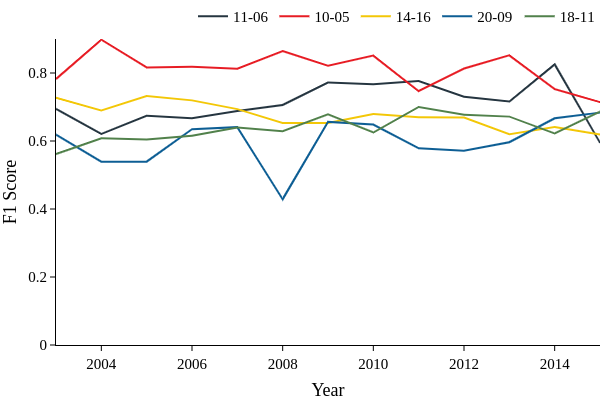
\includegraphics[width=\linewidth]{01.Chapters/05.Results/f1-combination-1-5}
		\caption{Correspondences 1 to 5.}
		\label{fig:top1-5}
	\end{subfigure}%
	\hfill
	\begin{subfigure}{0.49\textwidth}
		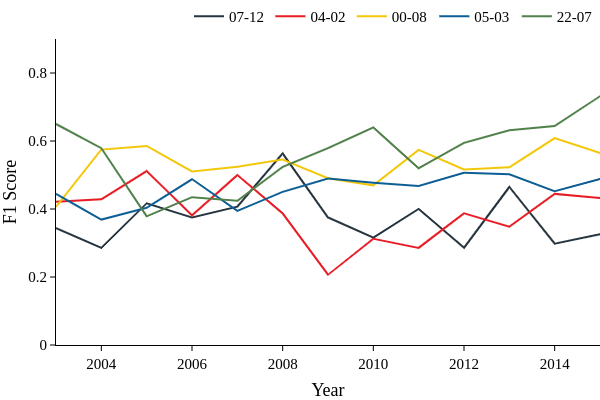
\includegraphics[width=\linewidth]{01.Chapters/05.Results/f1-combination-6-10}
		\caption{Correspondences 6 to 10.}
		\label{fig:top6-10}
	\end{subfigure}%
	\caption{F1 Score for the main correspondences.}
	\label{fig:f1-combination}
\end{figure}


% Comentar resultados das tabelas e dos gráficos
From Table \ref{tab:avg-combination-score}, we see a high negative correlation between the position of correspondences and their f1 scores, $-0.775$ for the record. This result said to us that is a decreasing relationship between the predictions of these correspondences. Figure \ref{fig:combination-corr} shows a scatter plot for this relationship with an ordinary least squares (OLS) trend line.

\begin{figure}[h!]
	\centering
	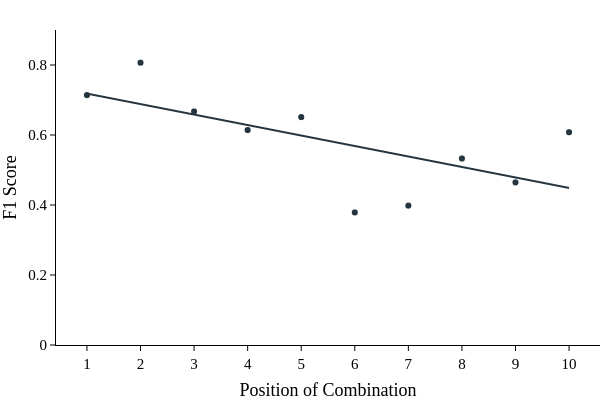
\includegraphics[width=0.6\linewidth]{01.Chapters/05.Results/combination-corr}
	\caption{F1 Score correlation with the correspondence position.}
	\label{fig:combination-corr}
\end{figure}

This decreasing trend reflects directly in score curves in Figure \ref{fig:f1-combination}. Despite slight fluctuations, the decreasing trend in correspondences scores could indicate that even in the best correspondences the predictions are not so accurate. The terms evolution over the years to develop the topics maybe have changed and the models can not learn these new terms.

Let us observe a little deeper at the relationship between the score and the time evolution. In Figure \ref{fig:isolated-topics} we have a scatter plot with the local regression trendline of LOWESS type for the two best correspondences. Notice that despite a small increase, there is a natural tendency of constancy followed by a decrease in the models' efficiency over the years. Again, this inclination suggests that the rising of new terms for new techniques affects the classification.

\begin{figure}[h!]
	\begin{subfigure}{0.5\textwidth}
	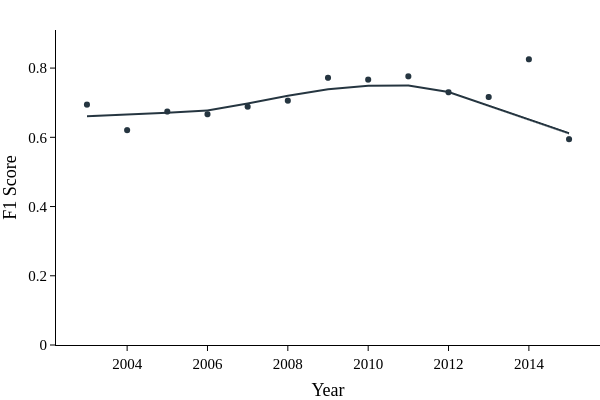
\includegraphics[width=\linewidth]{01.Chapters/05.Results/lowess-1}
		\caption{Topics correspondence \textit{Past 11} - \textit{Present 06}.}
	\end{subfigure}%
	\hfill
	\begin{subfigure}{0.5\textwidth}
		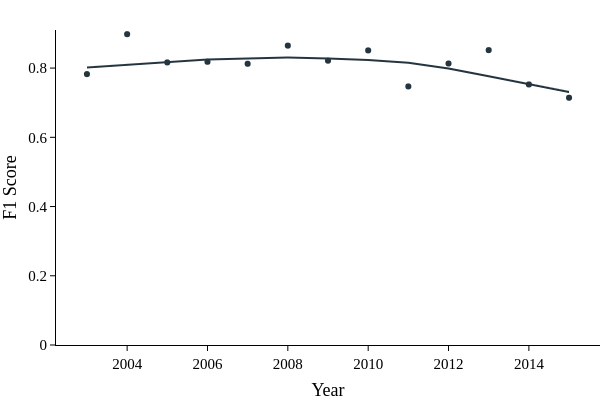
\includegraphics[width=\linewidth]{01.Chapters/05.Results/lowess-2}
		\caption{Topics correspondence \textit{Past 10} - \textit{Present 05}.}
	\end{subfigure}%
	\caption{F1 Score for the main correspondences.}
	\label{fig:isolated-topics}
\end{figure}

\newpage
Realize that correspondences under the top 5 may have some growth trend. However, in general, these correspondences already have low efficiency in relation to the best ones, decreasing the result's reliability.



%
%\chapter{Conclusions, Recommendations, and Future Works}\label{chap:conclusion}
%In this last chapter, we wrap up this work sharing conclusions. We also suggest new research lines inspired by the results of this work.

\section{Conclusions}

The main goal of this work was to evaluate the ability of classification models built from the topic modeling data, obtained by Latent Dirichelt Allocation. With a subset of documents, initial on time, called by \textit{Past}, we obtained their natural topics, then we do the same for intermediate data, called by \textit{Present}. After discovering the best combinations for these topics, we built classification models for each one of them and evaluate the predictions over the years.

In the chapter \ref{chap:intro}, we show a brief introduction, presenting the motivation and objective of this work. In chapter \ref{chap:literature} we described some important concepts of Natural Processing Language and classification techniques. In chapter \ref{chap:related} we presented related works that implement steps used in this work. 

Chapter \ref{chap:materials} described the whole methodology used to conduct the experimentation in this work, describing carefully each individual step. Finally, \ref{chap:results} presented and discussed the results obtained in each step of the experiment.

In synthesis, we saw from the results that is really possible to classify documents in short term, from a little subset of data. However, the topics evolve as time goes forward, evidenced by the discrepancy between the main closest combinations and those that follow right away.

We identified two aspects for these classification models. Firstly, we have a tendency of constancy in the efficiency of the model, because of the slow evolution of a given subject, mostly when dealing with scientific publications, as in our case. The second aspect shows a decreasing trend over time, as the model tends to unlearn about themes as new terms are used, such as neural networks, for example, recently the use of deep learning for these kinds of applications has become very popular.

Given this decreasing aspect, our models gradually lose their ability to predict. Therefore, a re-train routine could be fundamental to always keep achieving good results.

\section{Future Work}

From now, we propose other research lines some improvements directly by the results previously obtained:

\begin{itemize}
	\item \textit{Forecast Step:}
	
	The immediate continuation given the chronological order is develop the forecast step. Following the flowchart shown in Figure \ref{fig:forecast}, first, using the classifier we can build the incidence topic incidence matrix over time, with \textit{Past} and \textit{Present} sets. Then, apply a forecaster process for those time series with a Long Short-Term Memory neural network \cite{hochreiter1997long}. Finally, with the \textit{Future} set, perform an evaluation for the built forecaster.
	
	\begin{figure}[h!]
		\centering
		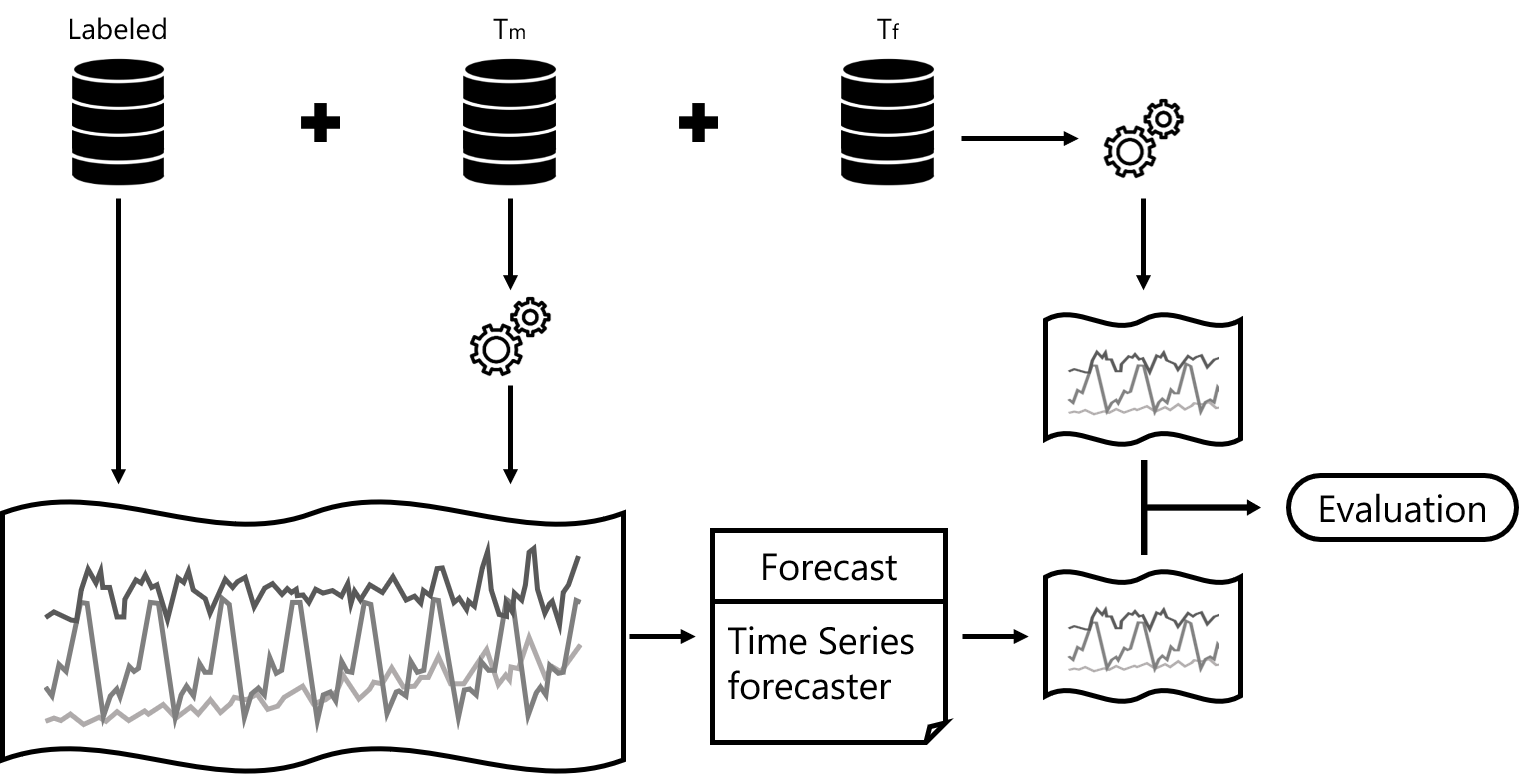
\includegraphics[width=0.8\linewidth]{01.Chapters/04.Materials/forecast}
		\caption{Flowchart to evaluate the time series model.}
		\label{fig:forecast}
	\end{figure}
	
	\item \textit{Retraining point:}
	
	Seeking to use this forecasting famework in a production enviroment, we will need to reduce the time granularity to month or even days. But, as we saw in Figure \ref{fig:isolated-topics} the classification models are losing efficiency over time. This research line aims to propose and evaluate metrics to identify an optimal threshold for retraining the topic model in order to uptade them with the new terms.
	
%	\item \textit{Topic modeling based on context:}
	
%	Text clusteing

	\item \textit{Feature extraction improvement:}
	
	In section \ref{sec:text-processing} we saw many techniques for normalization and vectorizing, but it doesn't stop there. There are several unexplored techniques that can improve our topic models and classification such as n-grams, hashing vectorizer and polinomial features, the word embedding itself presented a bad result due to the lack of a pre-trained model based on scientific publication context. This research line aims to use more sophisticated techniques for improve the topic and classification models, 
	
	
\end{itemize}


\chapter{The Proposal}\label{chap:proposal}
\section{Hypothesis}

\section{Objective}

\section{Research method}

\section{Schedule}


% REFERENCIAS BIBLIOGRAFICAS
\renewcommand\bibname{\itareferencesnamebabel} %renomear título do capítulo referências
\bibliography{02.Referencias/referencias}

% Apendices
%\appendix
%\chapter{}
%\input{}

% Anexos
%\annex
%\chapter{}
%\input{}

% Glossario
%\itaglossary
%\printglossary

% Folha de Registro do Documento
% Valores dos campos do formulario
\FRDitadata{June 19th, 2020}
\FRDitadocnro{DCTA/ITA/DM-018/2015} %(o n mero de registro voc  solicita a biblioteca)
\FRDitaorgaointerno{Aeronautics Institute of Technology -- ITA}
%Exemplo no caso de pós-graduação: Instituto Tecnol{\'o}gico de Aeron{\'a}utica -- ITA
\FRDitapalavrasautor{Natural Language Processing; Deep Learning; Machine Learning}
\FRDitapalavrasresult{Natural Language Processing; Deep Learning; Machine Learning}
%Exemplo no caso de gradua  o (TG):
%\FRDitapalavraapresentacao{Trabalho de Gradua  o, ITA, S o Jos  dos Campos, 2015. \NumPenultimaPagina\ p ginas.}

\FRDitapalavraapresentacao{ITA, São José dos Campos, 2020. Trabalho de Graduação. \NumPenultimaPagina\ páginas.}
\FRDitaresumo{Com avanço cientifico-tecnológico em escalas globais, a disponibilidade de dados para serem analisados cresce de maneira exponencial. A partir desse crescimento acelerado, técnicas de inteligência artificial, como o Processamento de Linguagem Natural (PLN), ajudam a automatizar o processo de se extrair informação de documentos.  Com intuito de realizar previsões sobre as tendências que surgirão em meio ao crescimento de dados, é possível utilizar técnicas de modelagem de tópicos para agrupar documentos em temas semelhantes e estudar a incidência temporal desses temas.

Assim, este trabalho busca aplicar técnicas de PLN combinadas com aprendizado supervisionado para agrupar documentos em um conjunto de temas e a partir disso aprender a identificá-los em novos documentos em um período futuro. Utilizando publicações cientificas da conferência de Sistemas de Processamento de Informação Neural, fomos capazes de modelar essa tarefa e obter bons resultados. Também estudamos a capacidade dos classificadores de manter desempenho satisfatório com o passar do tempo.
}
%  Primeiro Parametro: Nacional ou Internacional -- N/I
%  Segundo parametro: Ostensivo, Reservado, Confidencial ou Secreto -- O/R/C/S
\FRDitaOpcoes{N}{O}
% Cria o formulario
\itaFRD

\end{document}
% Fim do Documento. O massacre acabou!!! :-)
